

\chapter{Ordinary least squares regression}
\section{A line through the data}
Let's assume that a researcher wants to understand the relationship between two variables, $x$ and $y$, using a geometric line. Recall that a simple two dimensional line has two parameters, and intercept and a slope. In these notes, I call the intercept $\beta_0$ and the slope $\beta_1$ to form the function
\begin{equation}
\hat{y}_i=\beta_0+\beta_1x_i.
\end{equation}
Figure~\ref{fig:fit} is an example line. Note the hat above $y$ again, this lets us know that this is a prediction, not the actual value of $y$. The value of $\hat{y}_i$ is a {\it conditional mean}. If we wanted to show an expression for the actual value of $y$ for each case, we would need to show a residual, $e$, in the expression. This residual is the difference between the actual value of $y$ and the predicted value of $y$:
\begin{figure}
   \centering
   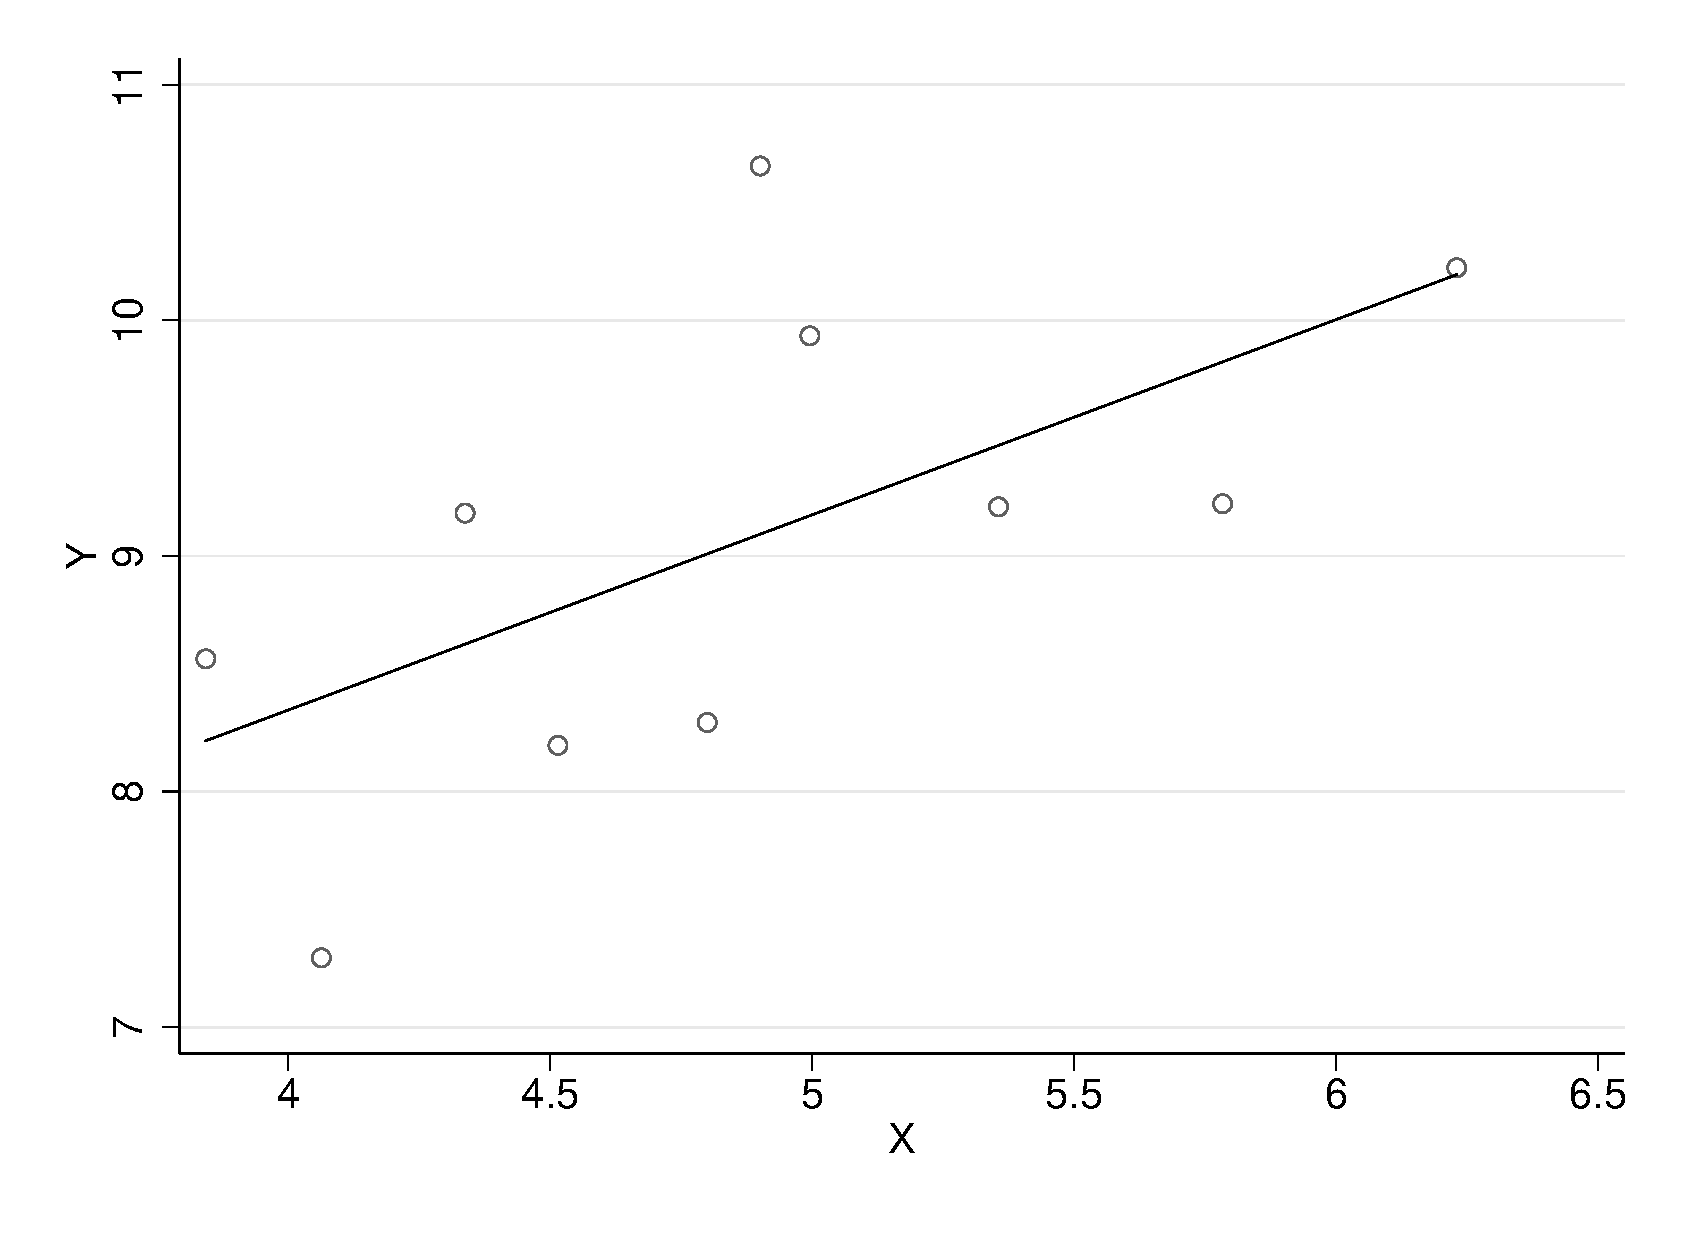
\includegraphics[angle=0,
           width=.75\textwidth]{fit.eps}
   \caption{Data from Table~\ref{tab:xy} fit with $\hat{y}_i=\beta_0+\beta_1x_i$.}
  \label{fig:fit}
\end{figure}
\begin{equation}
e_i=y_i-\hat{y}_i=y_i-\beta_0+\beta_1x_i
\end{equation}
It is also a deviation. Thus, the expression for the observed $y$ that includes the elements of the line is
\begin{equation}
y_i=\beta_0+\beta_1x_i+e_i.
\end{equation}
\begin{figure}
   \centering
   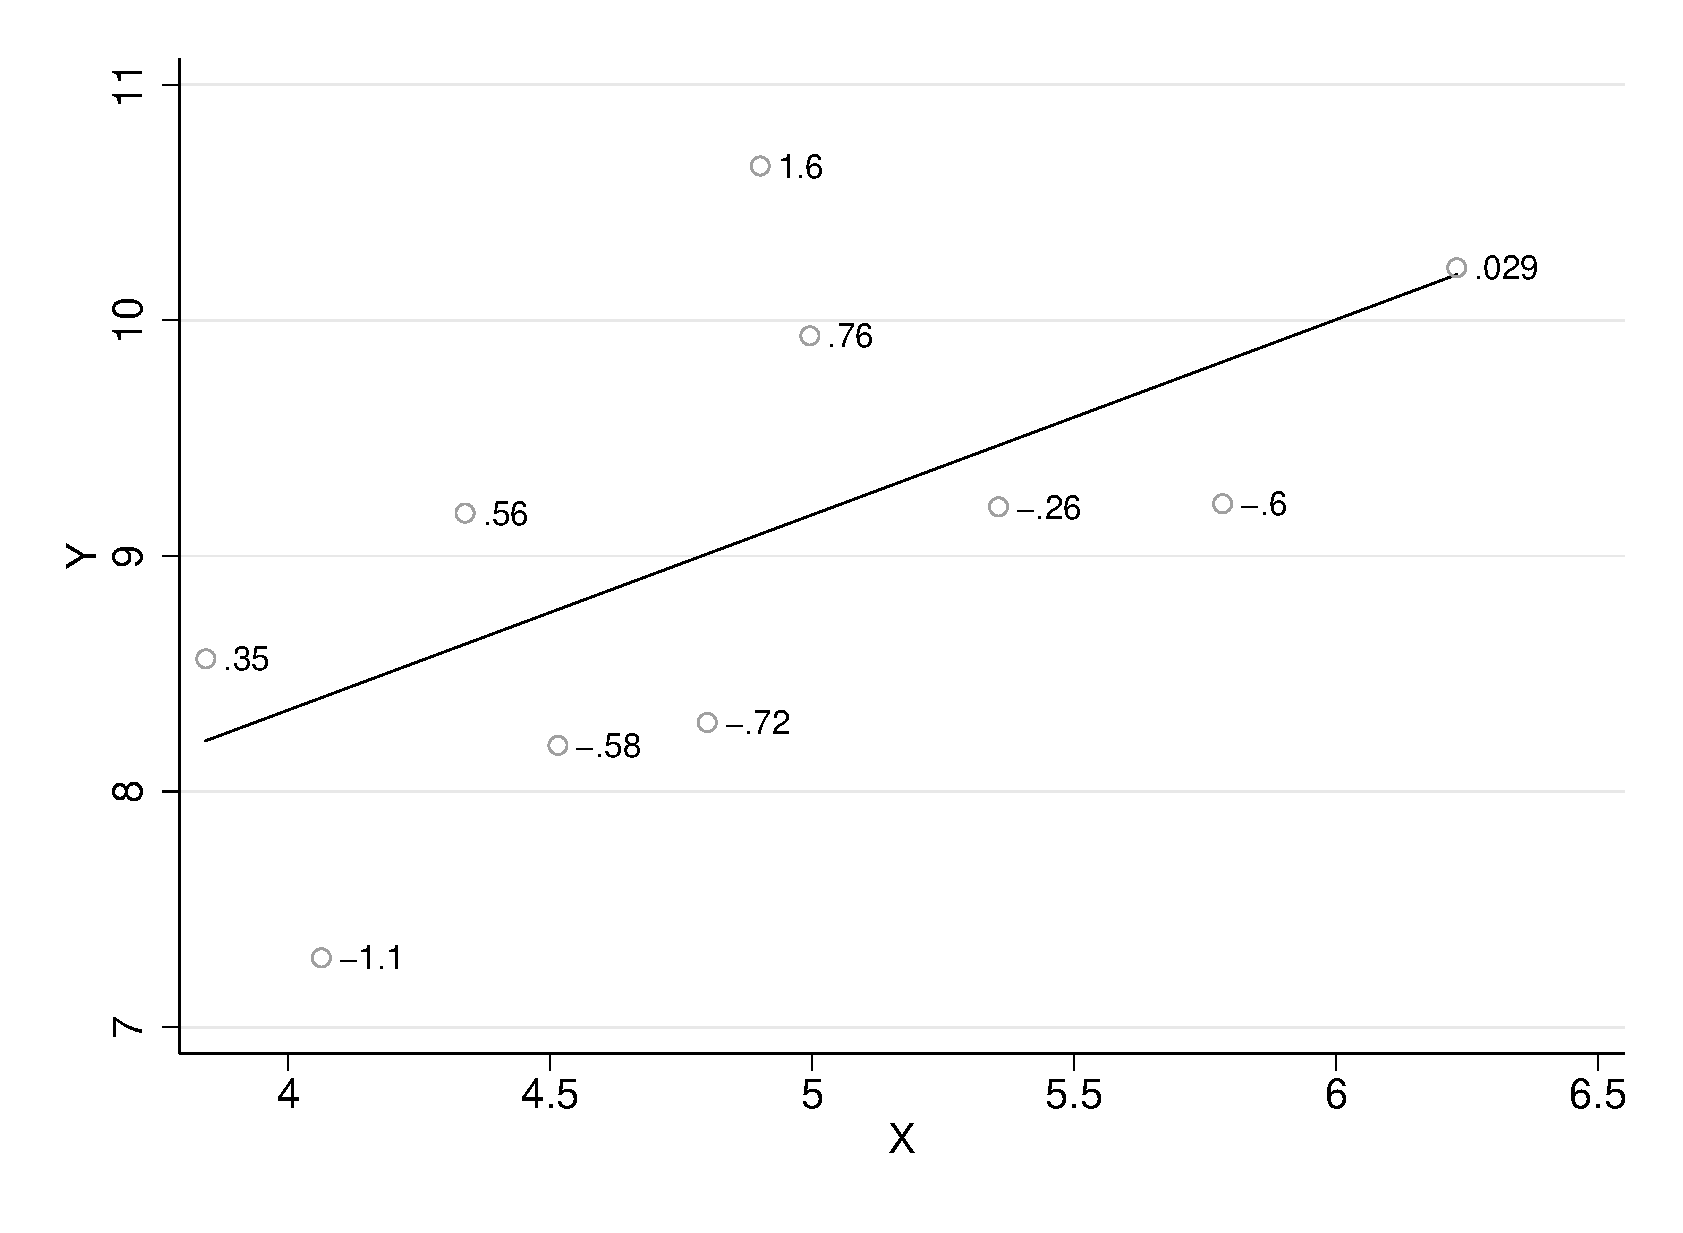
\includegraphics[angle=0,
           width=.75\textwidth]{efit.eps}
   \caption{Data from Table~\ref{tab:xy} fit with $\hat{y}_i=\beta_0+\beta_1x_i$ marked with the value of $e_i$.}
  \label{fig:efit}
\end{figure}
Figure~\ref{fig:efit} shows the residuals for each point on a scatterplot for the simulated data. Note how all the point below the regression line are negative, while all the points above the regression line are positive
\section{The regression slope}
Remember that correlation removes all information about the units of $x$ and $y$. Often, this is not useful to your average policy maker. They generally want to know, "if I put in one more unit of $x$, what happens to $y$?" In other words, if $x$ increases by one unit, what is the change in $y$ (and {\it in the units of $y$}).

We can do this with a regression slope. The formula for the regression slope is quite simple for bivaraite regression, and many parts should look familiar
\begin{equation}\label{eq:olsslope}
\beta_1=\frac{\sum_{i=1}^N\left(y_i-\bar{y}\right)\left(x_i-\bar{x}\right)}{\sum_{i=1}^N\left(x_i-\bar{x}\right)^2}
\end{equation}
Look back at the formula for correlation. This is exactly the same with one change: we removed the sum of squares for $y$ in the denominator. We interpret this statistic as the change in $y$ for a single unit increase in $x$.
\section{The intercept}
In order to draw a line we also need a $y$ intercept. The formula for this is also quite simple, With the slope in hand, we simply calculate the difference between the mean of $y$ and the mean of $x$ times the slope
\begin{equation}\label{eq:olsintercept}
\beta_0=\bar{y}-\beta_1\bar{x}
\end{equation}
This statistic tells us the predicted value of $y$ when $x$ is equal to 0. This will be very important later, as we can change the implicit meaning behind $x = 0$.
\section{Why is this the best fitting line?}
Where did this formula come from? The question to motivate this is: what line best summarizes the data? To answer this question, we need to operationalize what it means to best summarize the data, just as we did for the mean.

\subsection{Least squares formulation}

One idea is that we should first quantify the difference between what we observe for $y$ and what we predict for $y$. The deviation has previously been defined as $e_i$ for each case. Now, how can we summarize these differences in a single number? To do this, we once again return to the sum of squares. We summarize the deviation of the model from the observed as the sum of the squared residuals error ($SSE$)
\begin{equation}
SSE=\sum_{i=1}^Ne_i^2=\sum_{i=1}^N\left(y_i-\hat{y}_i\right)^2
\end{equation}
When $SSE$ is big, the model does a poor job predicting the data. When it's small, the model does a good job predicting the data. Intuitively, this should make sense. The closer the data are to the line, the smaller the $SSE$ will be and the further the data are away from the line, the larger the $SSE$ will be.

Now, how can we find the best line? We have a systematic way of finding the best line to fit the data. Here is the idea: we make $SSE$ a function of the slope and intercept:
\[
S\left(\beta_0,\beta_1\right)=\sum_{i=1}^Ne_i^2
\]
First, we replace the residual with what it is, the difference between $y$ and the regression line
\[
S\left(\beta_0,\beta_1\right)=\sum_{i=1}^N\left(y_i-\beta_0-\beta_1x_i\right)^2
\]
Next, we expand
\[
S\left(\beta_0,\beta_1\right)=\sum_{i=1}^N\left(y_i^2-2\beta_0y_i-2\beta_1y_ix_i+\beta_0^2+2\beta_0\beta_1x_i+\beta_1^2x_i^2\right)
\]
and pull the summations out
\[
S\left(\beta_0,\beta_1\right)=\sum_{i=1}^Ny_i^2-2\beta_0\sum_{i=1}^Ny_i-2\beta_1\sum_{i=1}^Ny_ix_i+N\beta_0^2+2\beta_0\beta_1\sum_{i=1}^Nx_i+\beta_1^2\sum_{i=1}^Nx_i^2
\]
We then find the partial derivative of $\beta_0$ (one of the two normal equations)
\[
\frac{\partial S}{\partial \beta_0}=2N\beta_0-2\sum_{i=1}^Ny_i-2\beta_1\sum_{i=1}^Nx_i
\]
and putting the elements back into the sum
\begin{equation}
\frac{\partial S}{\partial \beta_0}=-2\sum_{i=1}^N\left(y_i-\beta_0-\beta_1x_i\right)
\end{equation}
and the partial derivative of $\beta_1$ (the other normal equation)
\[
\frac{\partial S}{\partial \beta_1}=2\beta_0\sum_{i=1}^Nx_i+2\beta_1\sum_{i=1}^N-2\sum_{i=1}^Ny_ix_i
\]
and putting the elements back into the sum
\begin{equation}
\frac{\partial S}{\partial \beta_1}=-2\sum_{i=1}^N\left(y_i-\beta_0-\beta_1x_i\right)x_i
\end{equation}
We then set these both to 0, pull the constants out, and divide by $N$. That gives us for the intercept
\[
0=\bar{y}-\beta_0-\beta_1\bar{x}
\]
and for the slope
\[
0=\frac{1}{N}\sum_{i=1}^Nx_iy_i-\beta_0\bar{x}-\beta_1\frac{1}{N}\sum_{i=1}^Nx_i^2
\]
Two equations, two unknowns ($\beta_0$ and $\beta_1$). To get $\beta_1$, we figure that $\beta_0$ is
\[
\bar{y}-\beta_0-\beta_1\bar{x}=0
\]
\[
\beta_0=\bar{y}-\beta_1\bar{x}
\]
we then substitute $\bar{y}-\beta_1\bar{x}$ for $\beta_0$ in the second equation
\[
\frac{1}{N}\sum_{i=1}^Nx_iy_i-\beta_0\bar{x}-\beta_1\frac{1}{N}\sum_{i=1}^Nx_i^2 = 0
\]
\[
\frac{1}{N}\sum_{i=1}^Nx_iy_i-\left(\bar{y}-\beta_1\bar{x}\right)\bar{x}-\beta_1\frac{1}{N}\sum_{i=1}^Nx_i^2 = 0
\]
and solve for $\beta_1$
\[
\frac{1}{N}\sum_{i=1}^Nx_iy_i-\bar{y}\bar{x}+\beta_1\bar{x}^2-\beta_1\frac{1}{N}\sum_{i=1}^Nx_i^2 = 0
\]
\[
\frac{1}{N}\sum_{i=1}^Nx_iy_i-\bar{y}\bar{x} = -\beta_1\bar{x}^2+\beta_1\frac{1}{N}\sum_{i=1}^Nx_i^2
\]
\[
\frac{1}{N}\sum_{i=1}^Nx_iy_i-\bar{y}\bar{x} = \beta_1\left(-\bar{x}^2+\frac{1}{N}\sum_{i=1}^Nx_i^2\right)
\]
\[
\frac{\frac{1}{N}\sum_{i=1}^Nx_iy_i-\bar{y}\bar{x}}{\frac{1}{N}\sum_{i=1}^Nx_i^2-\bar{x}^2} = \beta_1
\]
which is the same as equation~\eqref{eq:olsslope}.

The data in Table~\ref{tab:xy} produced the regression in Table~\ref{tab:xyreg}. This is the best fit line. To demonstrate, I attempted to draw some other lines through the data, summed up the residuals, then plotted the $SSE$ for each line against the slope of that line in Figure~\ref{fig:altsse}.

\begin{table}[htbp]\centering
 \caption{Regression of $y$ on $x$ from data in Table~\ref{tab:xy}
\label{tab:xyreg}}
\begin{tabular}{lc}
Coefficients      &    Model  \\
\hline
$x$      &    0.829  \\
      &   (0.384)  \\
Intercept    &    5.032* \\
      &   (1.892)  \\
\hline
\multicolumn{1}{l}{$SE$s in parentheses, $*p<0.05$} \\
\hline
\end{tabular}
\end{table}

\begin{figure}
   \centering
   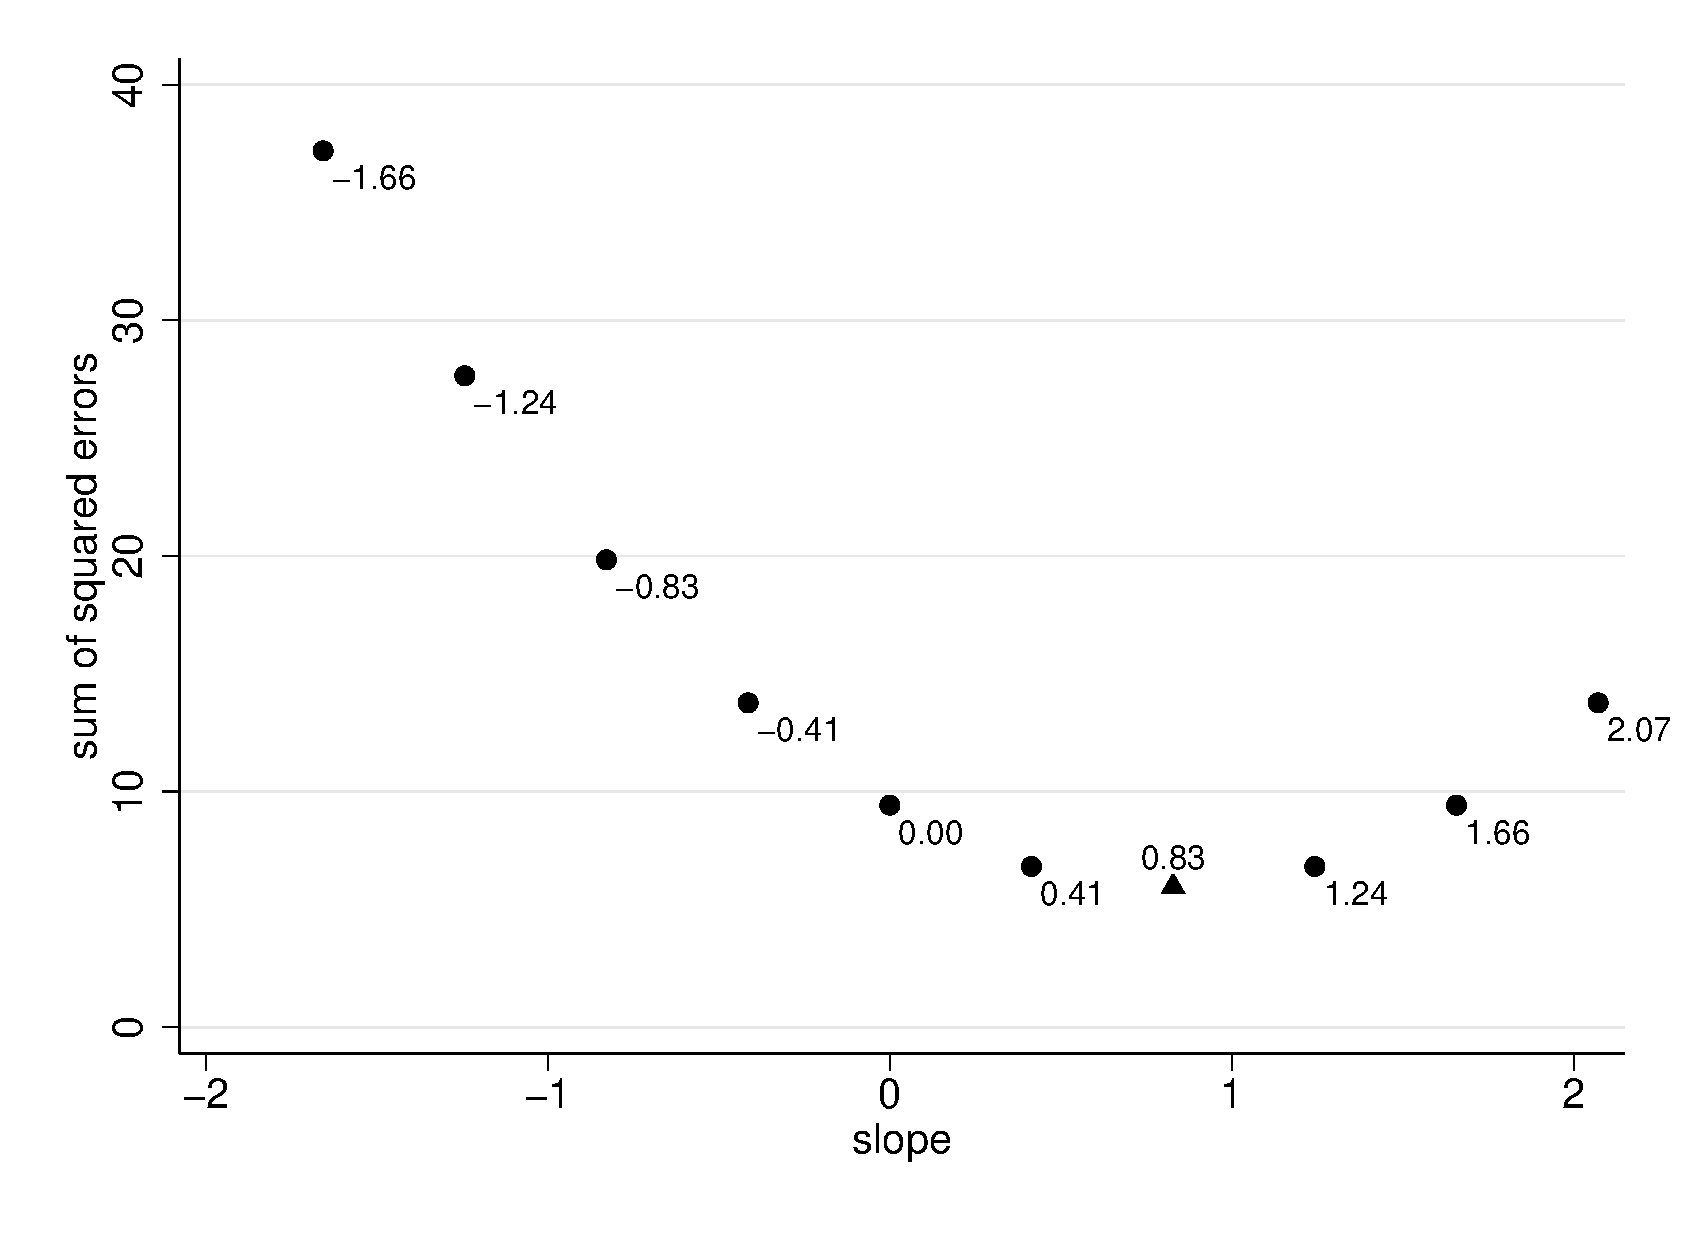
\includegraphics[angle=0,
           width=.75\textwidth]{altsse.eps}
   \caption{Alternate regression slopes and $SSE$s for data in Table~\ref{tab:xy}; real slope is 0.83.}
  \label{fig:altsse}
\end{figure}
What we find is that no matter what slope I use, I can't do better than the formulas provided here. Compare Figure~\ref{fig:sse} to Figure~\ref{fig:altsse} and you will see how regression works off the same least squares principle.

\subsection{Maximum likelihood formulation}

Another way to get to these estimates is to consider the likelihood of observing the data given the parameters. Since the predicted value $y$ is a conditional mean, we can start with the likelihood function of the mean
\begin{equation}
\mbox{ln}\left(L\left(\mu\vert y_1\ldots y_N\right)\right)=-\frac{1}{2}\sum_{i=1}^N\left(y_i-\mu\right)^2-\frac{N}{2}\left(\mbox{ln}\left(\sqrt{2\pi}\right)\right)
\end{equation}
and replace the mean with the regression formula
\begin{equation}
\mbox{ln}\left(L\left(\beta_0,\beta_1 \vert y_1\ldots y_N\right)\right)=-\frac{1}{2}\sum_{i=1}^N\left(y_i-\beta_0-\beta_1x_i\right)^2-\frac{N}{2}\left(\mbox{ln}\left(\sqrt{2\pi}\right)\right)
\end{equation}
and now we need to find the partial derivatives of this function, which look a lot like the least squares formulations. I won't do that all again, but hopefully you see that taking the derivatives of this function will produce the exact same estimators.  Thus, in this case, the least squares estimators are also the maximum likelihood estimators.

However, the only reason this works is because we assume a normal distribution. That is one of the assumptions of least squares: a normally distributed set of residuals. If that is not the case, then the maximum likelihood estimator will be different altogether, and then the least squares estimators will no longer be valid.
